% Options for packages loaded elsewhere
\PassOptionsToPackage{unicode}{hyperref}
\PassOptionsToPackage{hyphens}{url}
%
\documentclass[
]{article}
\usepackage{amsmath,amssymb}
\usepackage{CJKutf8} 
\usepackage{lmodern}
\usepackage{iftex}
\ifPDFTeX
  \usepackage[T1]{fontenc}
  \usepackage[utf8]{inputenc}
  \usepackage{textcomp} % provide euro and other symbols
\else % if luatex or xetex
  \usepackage{unicode-math}
  \defaultfontfeatures{Scale=MatchLowercase}
  \defaultfontfeatures[\rmfamily]{Ligatures=TeX,Scale=1}
\fi
% Use upquote if available, for straight quotes in verbatim environments
\IfFileExists{upquote.sty}{\usepackage{upquote}}{}
\IfFileExists{microtype.sty}{% use microtype if available
  \usepackage[]{microtype}
  \UseMicrotypeSet[protrusion]{basicmath} % disable protrusion for tt fonts
}{}
\makeatletter
\@ifundefined{KOMAClassName}{% if non-KOMA class
  \IfFileExists{parskip.sty}{%
    \usepackage{parskip}
  }{% else
    \setlength{\parindent}{0pt}
    \setlength{\parskip}{6pt plus 2pt minus 1pt}}
}{% if KOMA class
  \KOMAoptions{parskip=half}}
\makeatother
\usepackage{xcolor}
\IfFileExists{xurl.sty}{\usepackage{xurl}}{} % add URL line breaks if available
\IfFileExists{bookmark.sty}{\usepackage{bookmark}}{\usepackage{hyperref}}
\hypersetup{
  hidelinks,
  pdfcreator={LaTeX via pandoc}}
\urlstyle{same} % disable monospaced font for URLs
\usepackage{graphicx}
\makeatletter
\def\maxwidth{\ifdim\Gin@nat@width>\linewidth\linewidth\else\Gin@nat@width\fi}
\def\maxheight{\ifdim\Gin@nat@height>\textheight\textheight\else\Gin@nat@height\fi}
\makeatother
% Scale images if necessary, so that they will not overflow the page
% margins by default, and it is still possible to overwrite the defaults
% using explicit options in \includegraphics[width, height, ...]{}
\setkeys{Gin}{width=\maxwidth,height=\maxheight,keepaspectratio}
% Set default figure placement to htbp
\makeatletter
\def\fps@figure{htbp}
\makeatother
\setlength{\emergencystretch}{3em} % prevent overfull lines
\providecommand{\tightlist}{%
  \setlength{\itemsep}{0pt}\setlength{\parskip}{0pt}}
\setcounter{secnumdepth}{-\maxdimen} % remove section numbering
\ifLuaTeX
  \usepackage{selnolig}  % disable illegal ligatures
\fi

\author{}
\date{}

\begin{document}
\begin{CJK}{UTF8}{gbsn}
\textbf{宋伟任} 手机:18801910690

上海大学\textbar 工学硕士
邮箱:\href{mailto:songweiren_shu@163.com}{\nolinkurl{songweiren\_shu@163.com}}
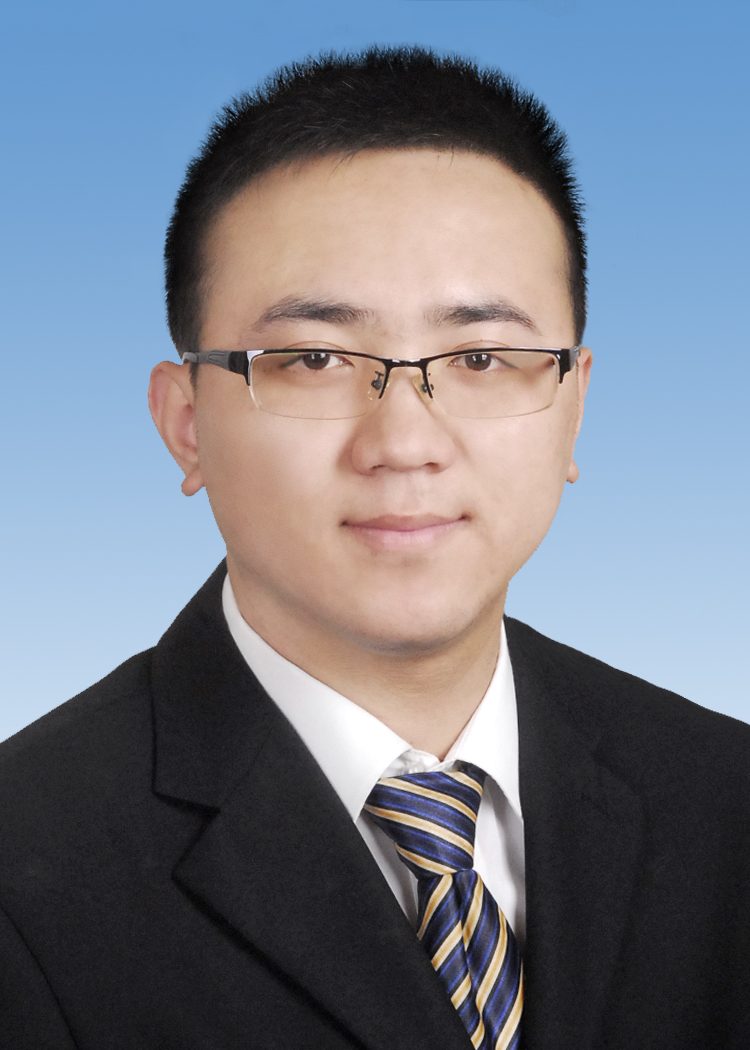
\includegraphics{./image/header.jpg}

出生年月:1992年4月

\textbf{PersonalSite}: \url{http://sfnr.top/}

\textbf{Github}: \url{https://github.com/DarrenSong}

\emph{\textbf{求职意向}} :软件工程师,算法工程师

2017年硕士研究生毕业,毕业后在云科伺服工作,主要负责在DSP2812平台上的通讯模块开发(C语言),熟悉工业现场总线,如MIII、CANOpen和TCP/IP等协议。一年后云科关门,到采埃孚作为一名电子软件工程师工作两年半,主要做TCU(汽车自动变速箱控制端元)应用层软件开发{[}C++{]},主控MCU是MPC5644,通讯协议以J1939为主。现在联影医疗担任软件开发工程师,主要负责Linux下CT系统的控制软件开发。本人熟悉C/C++、C\#和Python等编程语言,熟悉CC、Git、SVN等版本控制软件及DOORS,CQ和Integrity等需求管理软件,熟悉Vector工具链的开发及使用。熟悉Windows和Linux下程序开发,熟练使用VS2013/Source
Insight/CCS3.3/Keil5.0等IDE以及CMake和Shell脚本。本人勤奋努力,踏实好学,且有良好的团队意识,能够尽快的融入团队。

\begin{center}\rule{0.5\linewidth}{0.5pt}\end{center}

\hypertarget{ux6559ux80b2ux7ecfux5386}{%
\subparagraph{教育经历}\label{ux6559ux80b2ux7ecfux5386}}

\begin{center}\rule{0.5\linewidth}{0.5pt}\end{center}

    
        2010.9-2014.7
        上海大学  (机械工程及自动化)
        本科\textbar 学士
    
        
        2014.9-2017.6
        上海大学  (机械电子工程)
         研究生\textbar 硕士
    

\hypertarget{ux5de5ux4f5cux7ecfux5386}{%
\subparagraph{工作经历}\label{ux5de5ux4f5cux7ecfux5386}}

\begin{center}\rule{0.5\linewidth}{0.5pt}\end{center}

    
	    2021.3-至今
        上海联影医疗科技股份有限公司
        软件开发工程师
    
        
        2018.8-2021.2
        采埃孚(中国)投资有限公司
        电子软件工程师
    
        
        2017.6-2018.8
        云科智能伺服控制技术有限公司
        软件工程师
    

\hypertarget{ux9879ux76eeux7ecfux5386}{%
\subparagraph{项目经历}\label{ux9879ux76eeux7ecfux5386}}

\begin{center}\rule{0.5\linewidth}{0.5pt}\end{center}

\begin{itemize}
\item
  项目名称:伺服驱动器通信模块开发(云科智能伺服公司)

  项目描述:伺服驱动器主要用于CNC上三个加工轴的电机控制,介于CNC和电机之间,主控MCU是DSP2812。该项目主要是基于某种通讯协议{[}MIII/CANOpen{]}开发一款新的伺服驱动器。开发环境是CCS3.3编程语言为C语言,我负责实现通讯数据链路层及应用层的功能函数。主要分为以下几个部分,一是根据协议规范解析CNC下发的控制指令,并下发给控制层软件完成对应电机的控制,如加减速等;二是收集电机的状态信息比如转速,编码器值以及状态机信息组包成标准协议的报文上报给CNC系统。
\item
  项目名称:基于Windows的C++封包拦截工具(云科智能伺服公司)

  项目描述:开发环境是Qt,主要实现功能:捕获网卡数据,根据协议的报文结构解析从站的数据包
\item
  项目名称:基于Windows的伺服驱动器调试软件(云科智能伺服公司)

  项目描述:对于交付给客户的伺服驱动器,需要一并交付的是一个调式软件,能够对驱动器的一些参数进行修改,以便客户能够自己配置要使用的功能,因此开发上位机调试软件。开发环境为Visual
  Studio
  2015,编程语言为C\#(WinForm),上位机通过串口与驱动器进行通讯,协议为自定义协议,实现主要功能:在上位机界面提供修改电机控制模式的接口,以及调试电机常用的功能,如让电机进入使能状态,点动、连续运动等,以及一些PID整定参数的修改接口。
\item
  项目名称:TCU换挡策略调整(采埃孚)

  项目描述:在工程机械车辆上为了司机操作方便一般安装有两个换挡杆{[}一个是CAN协议跟TCU通讯,另一个输数字IO信号{]}用于车辆的换挡操作,但是同一时间TCU只接收来自其中一个挡杆的换挡请求。在我们现有基础上我实现了另外一套换挡逻辑。原有换挡逻辑为CAN
  Shift Lever 优先级较高,而FNR Lever
  优先级比较低,如果需要使用低优先级的lever,需要先把他的使能开关打开并且高优先级的lever在空挡。新的需求客户不希望使用使能开关,且不区分优先级,只要一个在空挡另外一个lever就可以完成相应的换挡请求。在代码中收到换挡请求以后不在判断不同lever的优先级,而是判断这两个换挡信号的一个组合信息,如果其中一个为空档,那么是一次有效的换挡请求,更新换挡策略,执行层执行相应的换挡操作。编写Unit
  test,进行SIL和HIL test,交付软件 。
\item
  项目名称:增加backup error memory(采埃孚)

  项目描述:对于一些分析变速箱故障比较关键的error
  code,我们不希望客户可以自己清除掉,以免造成分析困难。用10个word大小的eeprom
  作为Backup error memory,用于存储这些关键error
  code,这个地方存储的error我们不提供删除接口给客户。代码实现上给每个error分配一个Control
  word 的属性,通过配置这个值确定是否让此error 进入Backup error
  memory。在当前清除error函数中加入对error的control
  word的判断,如果是关键error,则除了存储在原来的地方外,另外再copy一份到Backup
  error memory。
\item
  项目名称:增加CAN message用于反馈TCU的IO信号(采埃孚)

  项目描述:在汽车上TCU除了通过CAN与ECU,CAN Shift
  lever以及VCU通信外,还有很多数字IO信号接收来自其他零部件的信号,如数字lever,刹车的角度信号和座位开关等。这些数字信号紧作为TCU内部使用,但是有些客户做自动驾驶功能需要多的信号来源,需要我们提供我们接收的数字信号。在代码实现方面,我将这些IO信号根据J1939协议标准组包为AUXIO1报文,周期性发送到CAN
  总线上,客户根据自己的需要从CAN message中读取解析相应的TCU IO信号。
\item
  项目名称:CT系统Gantry控制软件开发(联影医疗)

  项目描述:计算机断层扫描设备简称CT。我们组作为CT系统的Gantry控制软件开发部门,主要负责在扫描过程中对病床的移动控制,以及球管的放线停线控制,我主要负责球管的放线时间,放线时长以及放线功率的控制。软件开发平台是Linux,主要用C++开发。Gantry控制软件通过CANOpen与一块装有fpga的DCB板子通信,下发对球管的配置参数和控制指令,DCB板子通过SPI接口将参数和控制命令透传给球管控制模块,完成对球管的参数配置和停放线控制,球管的状态信号通过这条链路反向上报给我们Gantry控制软件。软件实现方面是基于boost的前向状态机通过定义不同的球管状态,完成对球管的不同状态的切换控制。
\end{itemize}

\hypertarget{ux4e13ux4e1aux6280ux80fd}{%
\subparagraph{专业技能}\label{ux4e13ux4e1aux6280ux80fd}}

\begin{center}\rule{0.5\linewidth}{0.5pt}\end{center}

C/C++、C\#、Python、Shell、makefile、markdown、数据结构与算法、Vector工具链(CANape,CANoe,CANalyzer)

\hypertarget{ux7efcux5408ux6280ux80fd}{%
\subparagraph{综合技能}\label{ux7efcux5408ux6280ux80fd}}

\begin{center}\rule{0.5\linewidth}{0.5pt}\end{center}

\begin{itemize}
\item
  语言能力 :中文(母语),英语(中级)
\item
  证书:全国计算机二级C语言,大学生节能减排大赛三等奖,普通话二级乙等
\item
  其他技能:C1驾照,ISTQB Certified Tester
\end{itemize}

*****English Version*****

\textbf{Weiren SONG} Phone:18801910690

Shanghai University\textbar{} Master
E-Mail:\href{mailto:songweiren_shu@163.com}{\nolinkurl{songweiren\_shu@163.com}}
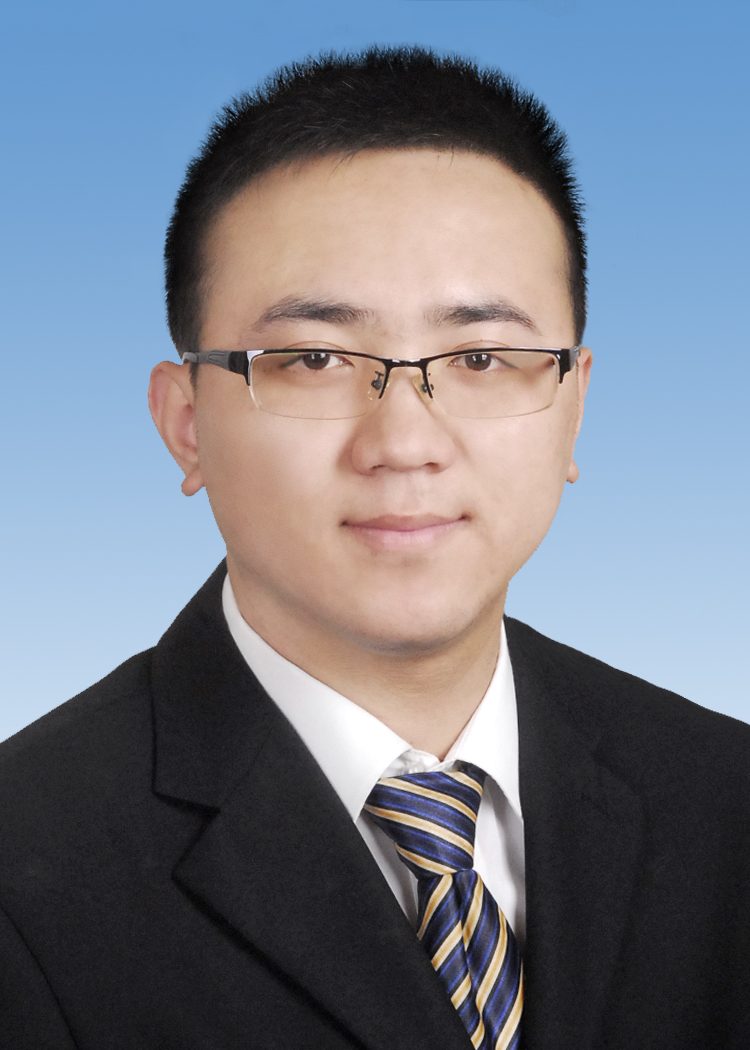
\includegraphics{./image/header.jpg}

birthday:1992.04

\textbf{PersonalSite}: \url{http://sfnr.top/}

\textbf{Github}: \url{https://github.com/DarrenSong}

\emph{\textbf{Job Intention}} :Software Engineer,Algorithm Engineer

I graduated with a master's degree in 2017 and worked in Yunke Servo
after graduation. I am mainly responsible for the development of
communication modules (C language) on the DSP2812 platform, and I am
familiar with industrial fieldbuses such as MIII, CANOpen and TCP/IP
protocols. One year later, Yunke closed, and worked at ZF as an
electronic software engineer for two and a half years, mainly doing TCU
(Automatic Transmission Control End Unit) application layer software
development {[}C++{]}, the main control MCU is MPC5644, the
communication protocol Mainly J1939. Now United Imaging Medical serves
as a software development engineer, mainly responsible for the control
software development of CT system under Linux. I am familiar with
programming languages such as C/C++, C\#, Python, etc., familiar with
version control software such as CC, Git, SVN, and demand management
software such as DOORS, CQ and Integrity, and familiar with the
development and use of Vector tool chain. Familiar with program
development under Windows and Linux, proficient in using VS2013/Source
Insight/CCS3.3/Keil5.0 and other IDEs, as well as CMake and Shell
scripts. I am diligent, practical, studious, and have a good sense of
teamwork. I can integrate into the team as soon as possible.

\begin{center}\rule{0.5\linewidth}{0.5pt}\end{center}

\hypertarget{education}{%
\subparagraph{Education}\label{education}}

\begin{center}\rule{0.5\linewidth}{0.5pt}\end{center}

    
        2010.9-2014.7
        Shanghai University  (Mechatronic Engineering \& Automation)
        Bachelor
    
        
        2014.9-2017.6
        Shanghai University  (Mechatronic \& Electric Engineering)
         Master
    

\hypertarget{work-experience}{%
\subparagraph{Work Experience}\label{work-experience}}

\begin{center}\rule{0.5\linewidth}{0.5pt}\end{center}

       
        2021.3-To Present
        United Imaging Healthcare Co., Ltd
        SW Engineer
    
        
        2018.8-To 2021.2
         ZF (China) Investment Co., Ltd.
        SW Engineer
    
        
		2017.6-2018.8
        YunKe Intelligent Servo Control Technology Co., Ltd.
        SW Engineer
    

\hypertarget{projects-experience}{%
\subparagraph{Projects Experience}\label{projects-experience}}

\begin{center}\rule{0.5\linewidth}{0.5pt}\end{center}

\begin{itemize}
\item
  Project Name:Develop the communication module of Servo driver(YunKe
  Servo)

  Description:The servo driver is mainly used for the motor control of
  the three machining axes on the CNC, which is between the CNC and the
  motor. The main control MCU is DSP2812. This project is mainly based
  on a certain communication protocol {[}MIII/CANOpen{]} to develop a
  new servo driver. The development environment is CCS3.3 programming
  language is C language, I am responsible for implementing the
  functions of the communication data link layer and the application
  layer. It is mainly divided into the following parts. One is to parse
  the control instructions issued by CNC according to the protocol
  specification, and send them to the control layer software to complete
  the control of the corresponding motor, such as acceleration and
  deceleration; the other is to collect the state information of the
  motor such as speed, code The device value and state machine
  information are packaged into standard protocol messages and reported
  to the CNC system.
\item
  Project Name:Sniffer Tool Via C++ based on Windows (YunKe Servo)

  Description:The IDE I used is Qt, I implement the coding for
  capturing the data and decode the data.
\item
  Project Name:Windows PC Software for config Servo driver(YunKe Servo)

  Description:For the servo drive delivered to the customer, a
  debugging software needs to be delivered together, which can modify
  some parameters of the drive, so that the customer can configure the
  functions to be used by himself, so the debugging software of the host
  computer is developed. The development environment is Visual Studio
  2015, the programming language is C\# (WinForm), the host computer
  communicates with the driver through the serial port, the protocol is
  a custom protocol, and the main functions are: Provide an interface to
  modify the motor control mode on the host computer interface, and
  debug the motor commonly used functions, such as letting the motor
  enter the enabled state, jogging, continuous motion, etc., as well as
  the modification interface of some PID tuning parameters
\item
  Project Name:Change the Gear shift strategy of TCU (ZF China)

  Description: On the construction machinery vehicle, two shift levers
  are generally installed for the convenience of the driver {[}one is
  the CAN protocol to communicate with the TCU, the other is the digital
  IO signal{]} for the vehicle's shifting operation, but at the same
  time the TCU only receives from one of them. Shift request for the
  lever. On our existing basis, I implemented another set of shifting
  logic. The original shift logic is that CAN Shift Lever has a higher
  priority, while FNR Lever has a lower priority. If you need to use a
  low-priority lever, you need to turn on his enable switch and the
  high-priority lever is in neutral. Customers with new requirements do
  not want to use the enable switch and do not differentiate the
  priority. As long as one is in neutral and the other is levered, the
  corresponding shift request can be completed. After receiving the
  shift request in the code, it does not judge the priority of different
  levels, but judges a combination of the two shift signals. If one of
  them is neutral, it is a valid shift request, and the shift is
  updated. Strategy, the execution layer performs the corresponding
  shift operation. Write Unit tests, conduct SIL and HIL tests, and
  deliver software.
\item
  Project Name:add the backup error memory for TCU (ZF China)

  Description:For some error codes that are critical for analyzing
  gearbox failures, we do not want customers to clear them by
  themselves, so as not to cause difficulties in analysis. A 10-word
  eeprom is used as the Backup error memory to store these key error
  codes. We do not provide a delete interface for the errors stored in
  this place. The code implementation assigns an attribute of Control
  word to each error, and determines whether to let the error enter the
  Backup error memory by configuring this value. Add the judgment of the
  control word of the error to the current clear error function. If it
  is a key error, in addition to storing it in the original place,
  another copy is copied to the Backup error memory.
\item
  Project Name:add a broadcast CAN message from J1939(AUXIO1) (ZF
  China)

  Description:In the car, in addition to communicating with ECU, CAN
  Shift lever and VCU through CAN, TCU also has many digital IO signals
  to receive signals from other components, such as digital lever, brake
  angle signal and seat switch. These digital signals are strictly used
  inside the TCU, but some customers need more signal sources for
  automatic driving functions, and we need to provide the digital
  signals we receive. In terms of code implementation, I package these
  IO signals into AUXIO1 messages according to the J1939 protocol
  standard, and send them to the CAN bus periodically. Customers can
  read and parse the corresponding TCU IO signals from the CAN message
  according to their own needs.
\item
  Project Name:Develop Gantry SW of CT System (UIH)

  Description:Computed tomography is abbreviated as CT. As the Gantry
  control software development department of the CT system, our group is
  mainly responsible for the movement control of the patient bed during
  the scanning process, as well as the control of the tube's line
  release and stop line. I am mainly responsible for the tube line
  release time, line release time and line release. power control. The
  software development platform is Linux, which is mainly developed in
  C++. Gantry control software communicates with a DCB board equipped
  with fpga through CANOpen, and issues configuration parameters and
  control instructions for the tube. Parameter configuration and parking
  line control, the status signal of the tube is reversely reported to
  our Gantry control software through this link. In terms of software
  implementation, the forward state machine based on boost completes the
  switching control of different states of the tube by defining
  different states of the tube.
\end{itemize}

\hypertarget{professional-skills}{%
\subparagraph{Professional Skills}\label{professional-skills}}

\begin{center}\rule{0.5\linewidth}{0.5pt}\end{center}

C/C++、C\#、Python、Shell、makefile、markdown、Data Structures And
Algorithms、VectorTools(CANape,CANoe,CANalyzer)

\hypertarget{integrated-skills}{%
\subparagraph{Integrated Skills}\label{integrated-skills}}

\begin{center}\rule{0.5\linewidth}{0.5pt}\end{center}

\begin{itemize}
\item
  Language :Chinese, English
\item
  Certificate:National Computer Rank Examination, Energy Saving
  \&Emission Reduction
\item
  Other Skills:C1 driving license, ISTQB Certified Tester
\end{itemize}
\end{CJK}

\end{document}
